\documentclass[11pt,a4paper,dvipdfmx]{jlreq}

% 必須パッケージ
\usepackage[dvipdfmx]{graphicx} % 画像読み込み
\usepackage{caption}            % minipage内でキャプションをつけるため
\usepackage{amsmath,amssymb}
\usepackage{url}

% ページ余白の調整（図を大きく見せるため少し余白を狭くする設定）
\usepackage[top=25mm, bottom=25mm, left=20mm, right=20mm]{geometry}

% タイトル情報
\title{CO$_2$貯留・放散装置向け制御基板(M304)用ファームウェア仕様書}
\author{氏名}
\date{\today}

\begin{document}

\maketitle

\begin{abstract}
本ドキュメントは，CO$_2$貯留・放散装置向け制御基板(M304)用の主要なファームウェアロジックの仕様についてまとめたものである．
各モジュールの処理フローを可視化し，システム全体の挙動を定義する．
\end{abstract}

\tableofcontents
\clearpage

% ==========================================
\section{メイン制御ループ (\texttt{main.ino})}

\noindent
% 左側のブロック（幅を全体の55%に設定）
\begin{minipage}[t]{0.55\textwidth}
    \vspace{0pt} % 上端を揃えるためのおまじない
    \centering
    % 高さをテキスト領域の85%に制限してページオーバーを防ぐ
    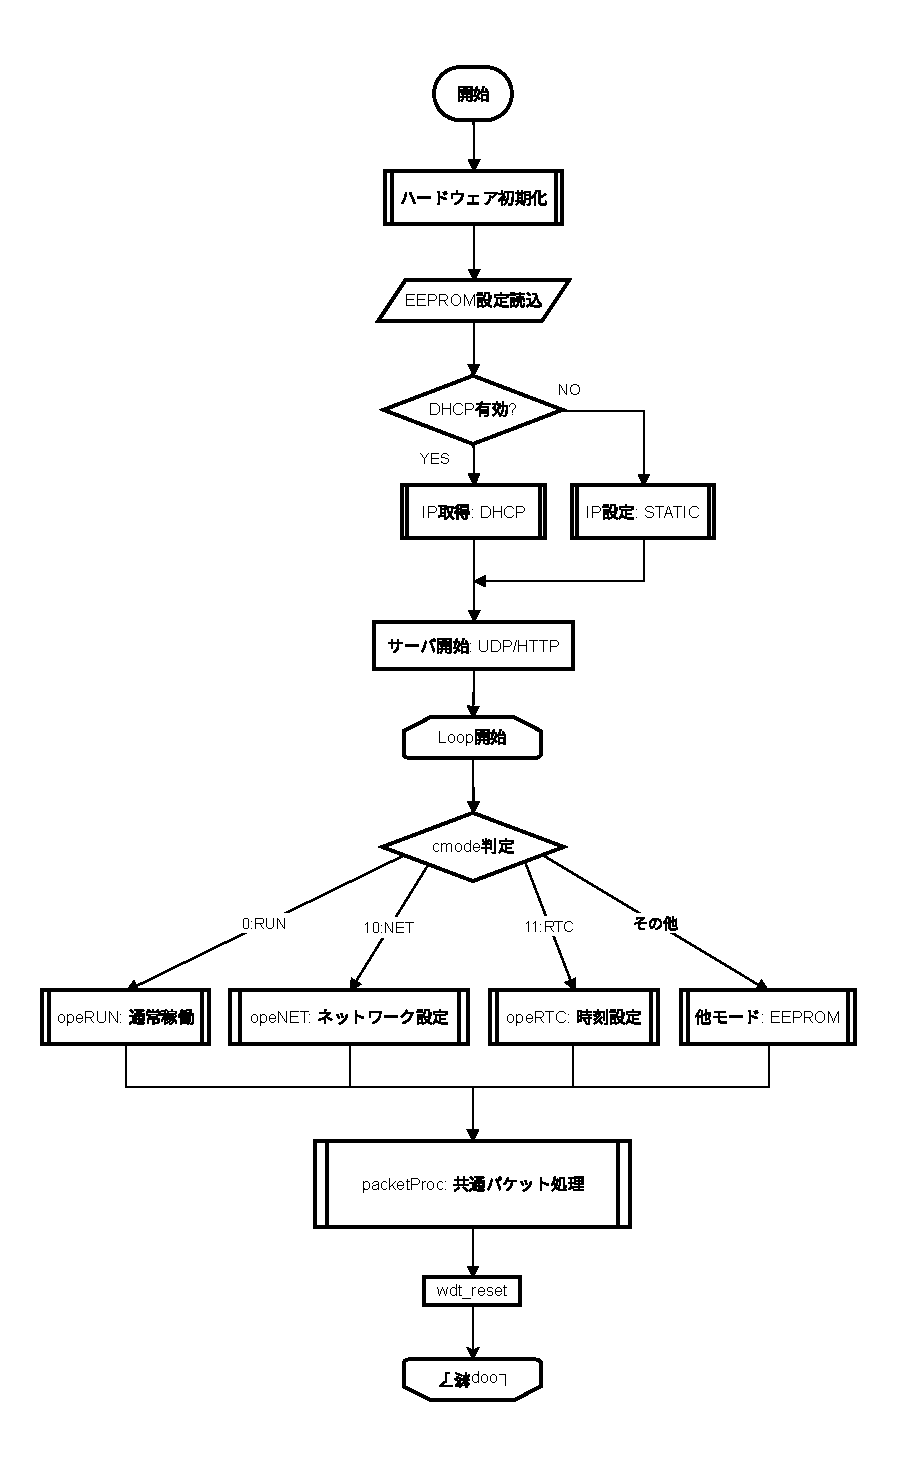
\includegraphics[width=\linewidth, height=0.85\textheight, keepaspectratio]{main_ino.drawio.pdf}
    \captionof{figure}{\texttt{main.ino} の全体処理フロー}
    \label{fig:main}
\end{minipage}
\hfill
% 右側のブロック（幅を全体の40%に設定）
\begin{minipage}[t]{0.4\textwidth}
    \vspace{0pt}
    システムの起動から初期化，および定常状態におけるメインループの処理フローを左図に示す．．
    
    ハードウェア初期化後，EEPROM から設定を読み込み，ネットワークの確立を経て自律制御ループへと移行する．．DHCP の有効・無効によって IP アドレスの取得方法が分岐し，最終的に UDP/HTTP サーバが立ち上がる．．
    
    ループ開始後は \texttt{cmode} 変数の値に従い，各機能（\texttt{opeRUN}, \texttt{opeNET}, \texttt{opeRTC} 等）の処理へディスパッチされ，最後に \texttt{packetProc} による共通パケット処理とウォッチドッグタイマー（WDT）のリセットが行われる．．
\end{minipage}

\clearpage % ページを強制的に分割

% ==========================================
\section{自動制御・データ送信 (\texttt{opeRUN()})}

\noindent
\begin{minipage}[t]{0.55\textwidth}
    \vspace{0pt}
    \centering
    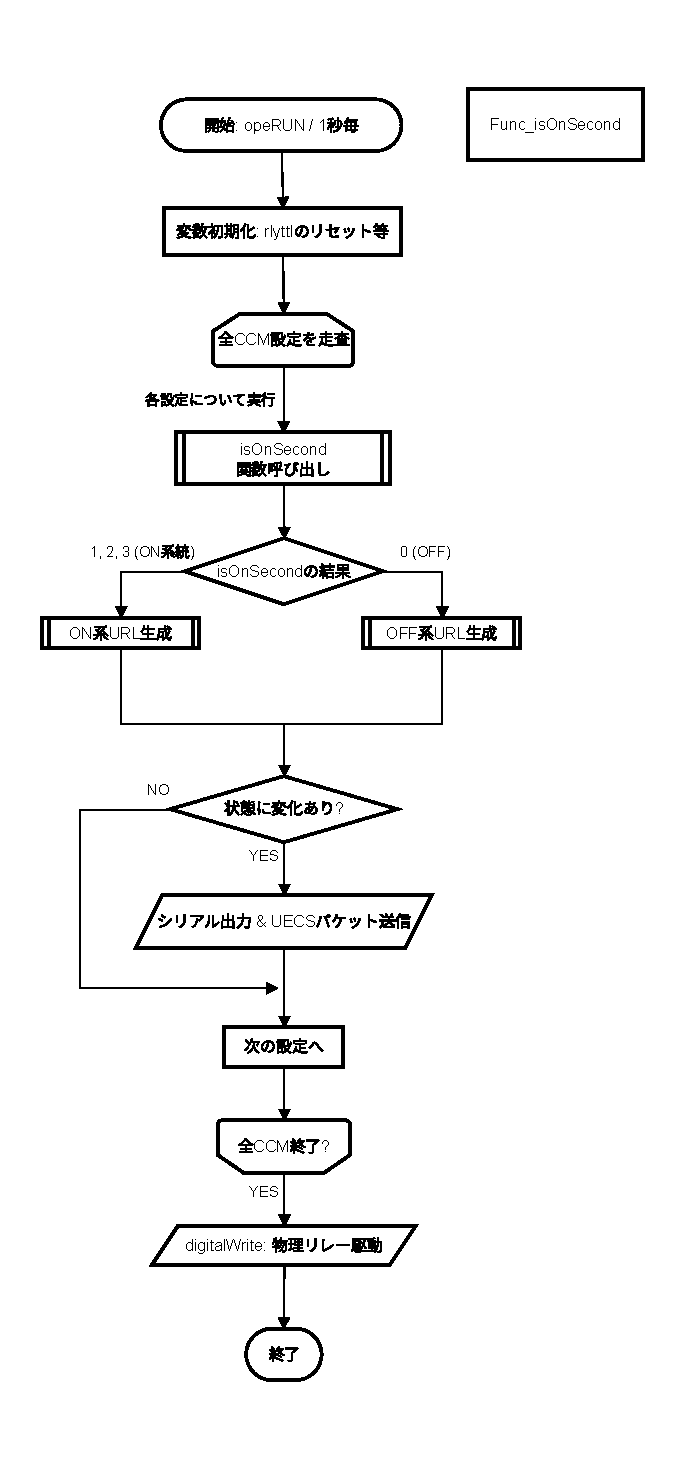
\includegraphics[width=\linewidth, height=0.85\textheight, keepaspectratio]{opeRUN_ino.drawio.pdf}
    \captionof{figure}{\texttt{opeRUN()} の制御および送信フロー}
    \label{fig:operun}
\end{minipage}
\hfill
\begin{minipage}[t]{0.4\textwidth}
    \vspace{0pt}
    \texttt{opeRUN()} 関数は，本システムの主目的である「環境制御の自動実行」と「データ計測・配信」を担う中心的なモジュールである．．

    処理は大きく分けて以下の2段階で構成される：．
    
    \begin{enumerate}
        \item \textbf{自律リレー制御}:．\\
        内蔵 RTC (Real Time Clock) から取得した現在時刻に基づき，各リレーに対応するスケジュール設定を評価する．．ここで前述の \texttt{isOnSecond()} が呼び出され，1秒単位の精度で物理的なハードウェア操作が実行される．．
        
        \item \textbf{UECS データの送出}:．\\
        EEPROM 内の TX CCM（送信設定）テーブルを走査し，規定のインターバル（通常1秒間隔）ごとに，自ノードの計測値や動作状態を UECS 規格の XML パケットとしてネットワークへ送出する．．
    \end{enumerate}

    このループを繰り返すことで，外部サーバに依存しない独立した自律制御と，UECS 規格による相互監視・記録の両立を実現している．．
\end{minipage}

\clearpage

% ==========================================
\section{自律制御ロジック (\texttt{isOnSecond()})}

\noindent
\begin{minipage}[t]{0.55\textwidth}
    \vspace{0pt}
    \centering
    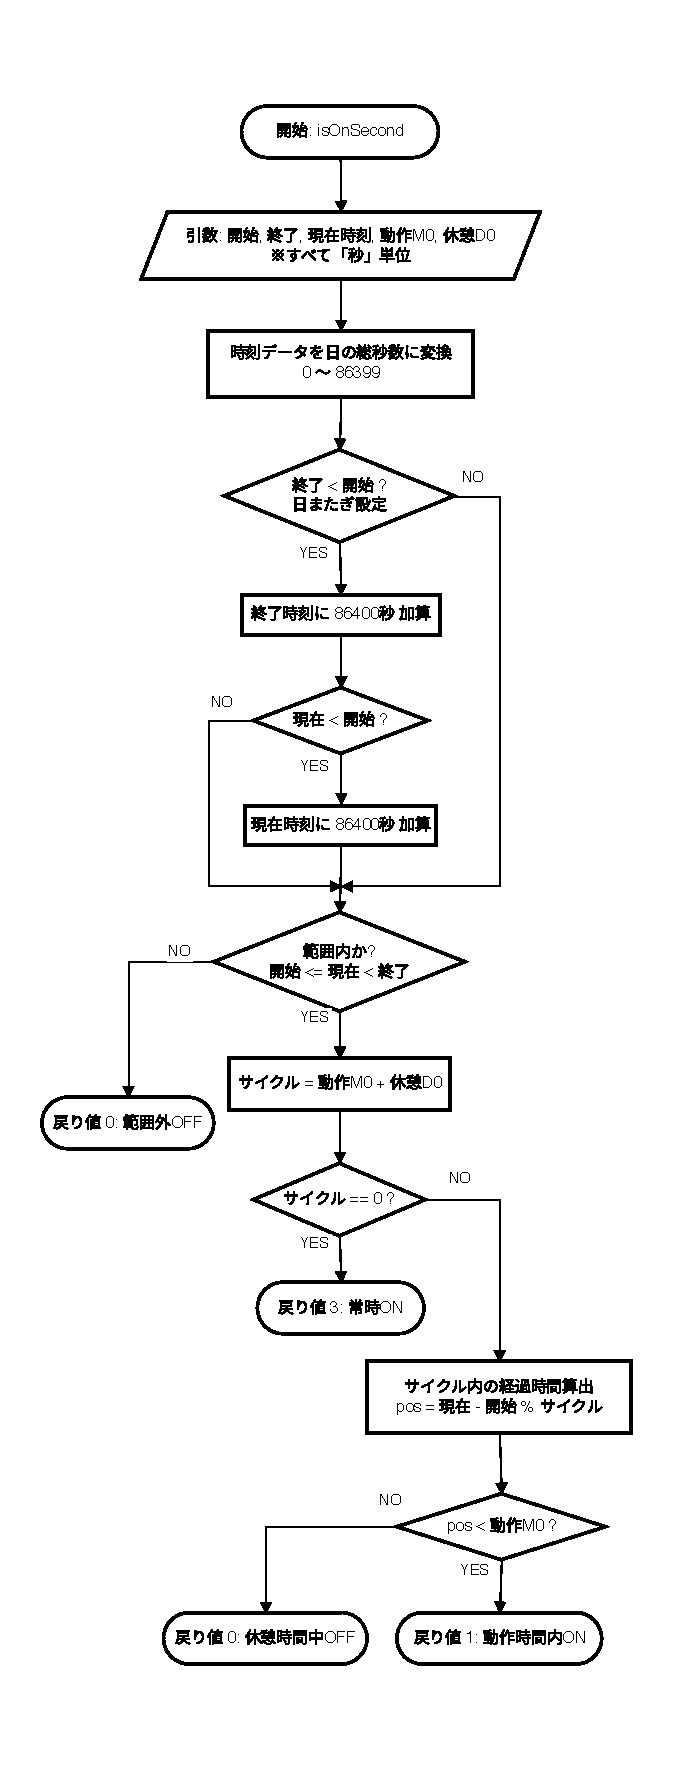
\includegraphics[width=\linewidth, height=0.85\textheight, keepaspectratio]{isOnSecond.drawio.pdf}
    \captionof{figure}{\texttt{isOnSecond()} 関数の判定ロジック}
    \label{fig:ison}
\end{minipage}
\hfill
\begin{minipage}[t]{0.4\textwidth}
    \vspace{0pt}
    本システムにおけるアクチュエータの動作判定は，秒単位の高精度な計算によって行われる．．
    
    従来バージョンの分単位判定から改良され，1日の総秒数（86400秒）を基準とすることで，日またぎの動作や微細な間欠動作を正確に処理する設計となっている．．
    
    引数として与えられた開始時刻と終了時刻を秒単位の整数値に正規化し，現在時刻がその範囲内に収まっているかを判定する．．範囲内の場合，さらに動作時間（\texttt{M0}）と休憩時間（\texttt{D0}）を加算したサイクル時間を算出し，現在の経過時間が動作時間内であるかによって最終的な ON/OFF（戻り値 1 または 0）を決定する．．
\end{minipage}

\clearpage

% ==========================================
\section{ネットワーク管理 (\texttt{opeNET()})}

\noindent
\begin{minipage}[t]{0.55\textwidth}
    \vspace{0pt}
    \centering
    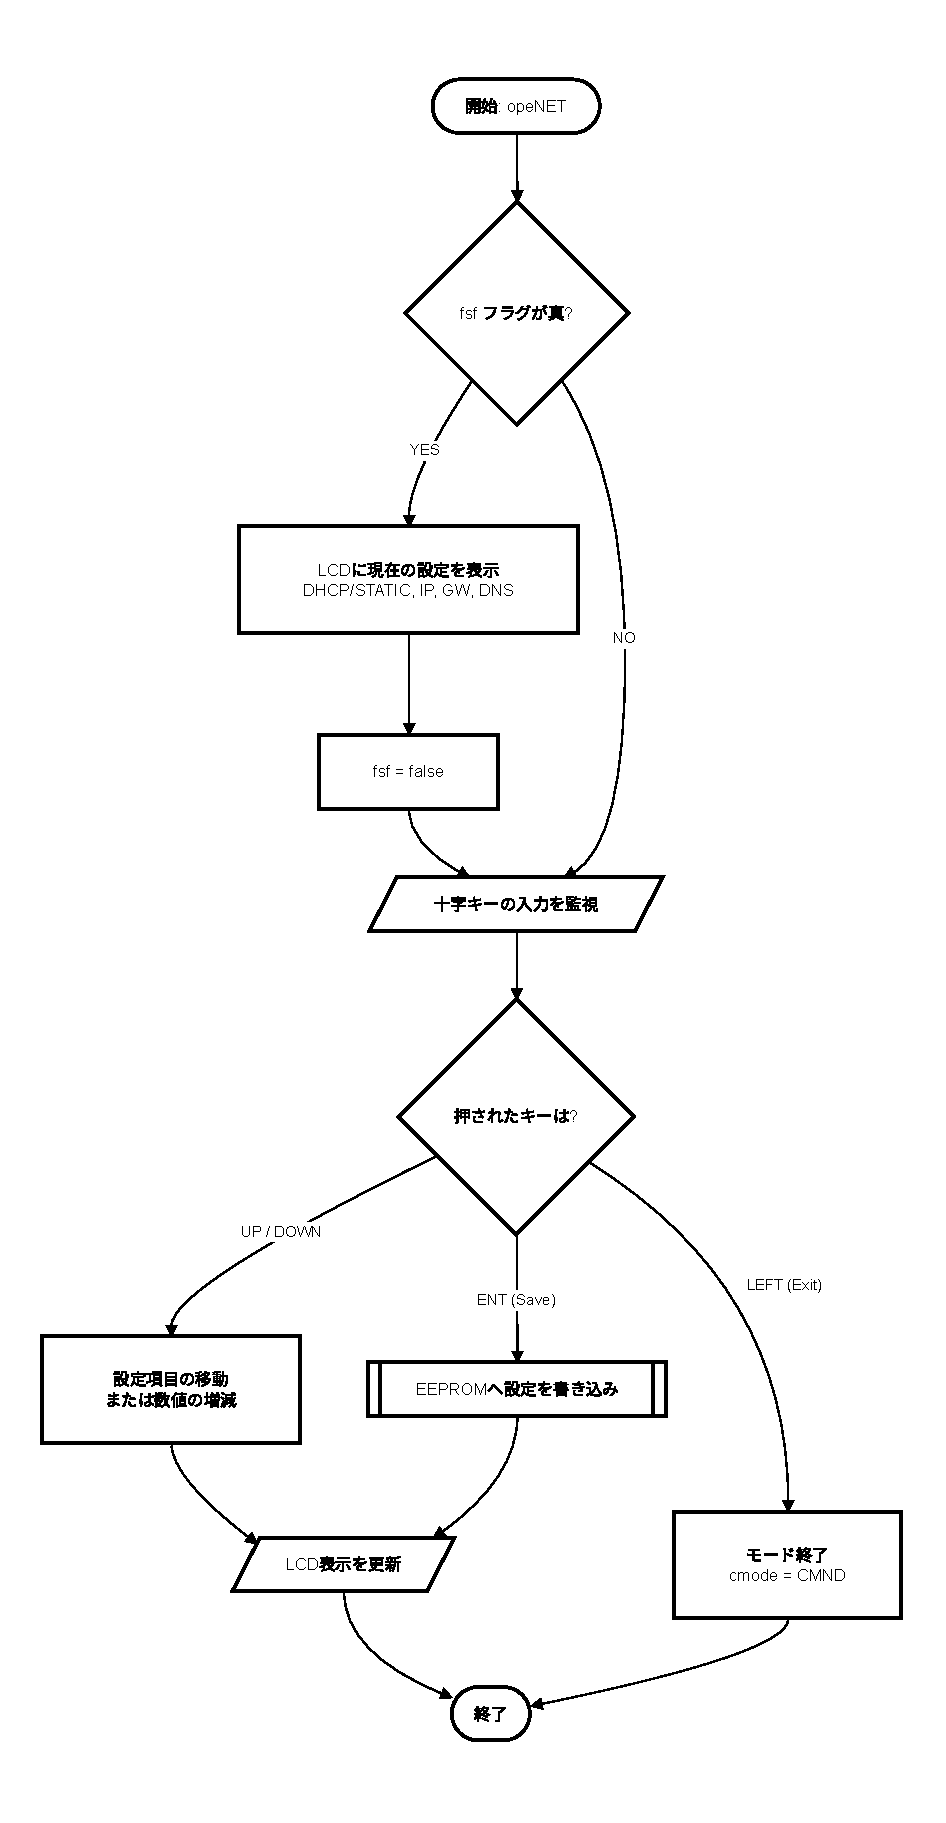
\includegraphics[width=\linewidth, height=0.85\textheight, keepaspectratio]{opeNET_ino.drawio.pdf}
    \captionof{figure}{\texttt{opeNET()} のネットワーク初期化フロー}
    \label{fig:openet}
\end{minipage}
\hfill
\begin{minipage}[t]{0.4\textwidth}
    \vspace{0pt}
    \texttt{opeNET()} 関数は，Ethernet W5500 コントローラを制御し，本システムが UECS ネットワーク内で通信を行うための物理層およびネットワーク層のセットアップを行うモジュールである．．

    本モジュールの主な特徴は以下の通りである：．
    
    \begin{itemize}
        \item \textbf{柔軟なアドレス割り当て}:．\\
        EEPROM 内の設定フラグを参照し，DHCP による動的取得と，あらかじめ指定された固定 IP アドレスの適用を切り替える．．
        \item \textbf{堅牢な接続性}:．\\
        DHCP による取得に失敗した場合には，即座にデフォルトの固定 IP 設定を適用するフォールバック機能を備えており，ネットワークトラブル時でもノードの完全な孤立を防ぐ設計となっている．．
        \item \textbf{サービス起動}:．\\
        IP アドレス確定後，UECS 通信に必要な UDP ポートのリスニングおよび，Web 設定画面を提供するための HTTP サーバーを起動する．．
    \end{itemize}

    本処理は主に起動時および，設定変更によるネットワーク再起動要求が発生した際に実行される．．
\end{minipage}

\clearpage

% ==========================================
\section{通信・パケット処理 (\texttt{packetProc()})}

\noindent
\begin{minipage}[t]{0.6\textwidth} % 横幅が広い図の場合は比率を変える
    \vspace{0pt}
    \centering
    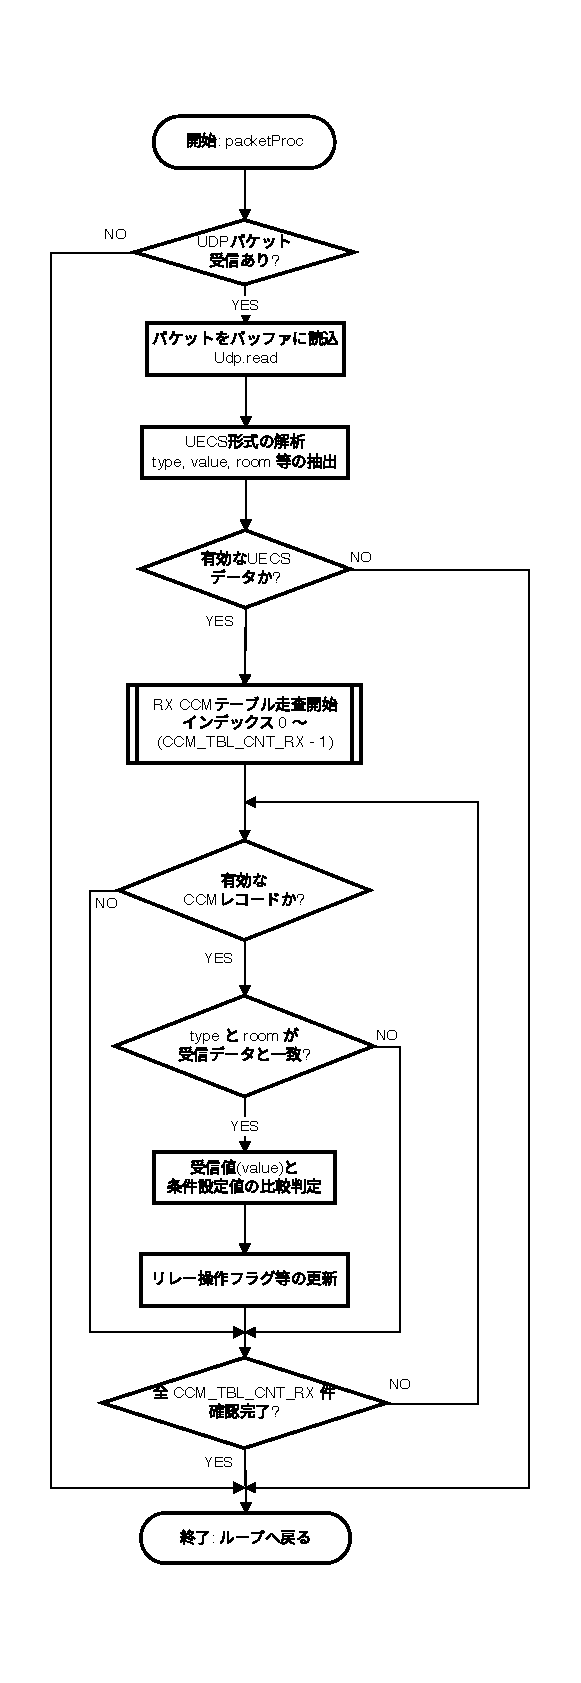
\includegraphics[width=\linewidth, height=0.85\textheight, keepaspectratio]{packetProc.drawio.pdf}
    \captionof{figure}{\texttt{packetProc()} における処理手順}
    \label{fig:packet}
\end{minipage}
\hfill
\begin{minipage}[t]{0.35\textwidth}
    \vspace{0pt}
    外部ノードからの制御要求やセンサ値のブロードキャストを受信する処理を左図に示す．．
    
    本処理はノンブロッキングで設計されており，UDP パケットが到達していない場合は即座に処理を返す．．パケットを受信した場合は UECS 規格に基づいてデータを抽出し，EEPROM から展開された RX CCM テーブル（最大 \texttt{CCM\_TBL\_CNT\_RX} 件）と順次照合する．．
    
    \texttt{type} および \texttt{room} が合致した場合，設定された条件式による比較判定を行い，対応するリレー操作フラグを更新することで，他ノードと連動した協調動作を実現している．．
\end{minipage}

\clearpage

\end{document}
